\documentclass{beamer}\usepackage[]{graphicx}\usepackage[]{color}
%% maxwidth is the original width if it is less than linewidth
%% otherwise use linewidth (to make sure the graphics do not exceed the margin)
\makeatletter
\def\maxwidth{ %
  \ifdim\Gin@nat@width>\linewidth
    \linewidth
  \else
    \Gin@nat@width
  \fi
}
\makeatother

\definecolor{fgcolor}{rgb}{0.345, 0.345, 0.345}
\newcommand{\hlnum}[1]{\textcolor[rgb]{0.686,0.059,0.569}{#1}}%
\newcommand{\hlstr}[1]{\textcolor[rgb]{0.192,0.494,0.8}{#1}}%
\newcommand{\hlcom}[1]{\textcolor[rgb]{0.678,0.584,0.686}{\textit{#1}}}%
\newcommand{\hlopt}[1]{\textcolor[rgb]{0,0,0}{#1}}%
\newcommand{\hlstd}[1]{\textcolor[rgb]{0.345,0.345,0.345}{#1}}%
\newcommand{\hlkwa}[1]{\textcolor[rgb]{0.161,0.373,0.58}{\textbf{#1}}}%
\newcommand{\hlkwb}[1]{\textcolor[rgb]{0.69,0.353,0.396}{#1}}%
\newcommand{\hlkwc}[1]{\textcolor[rgb]{0.333,0.667,0.333}{#1}}%
\newcommand{\hlkwd}[1]{\textcolor[rgb]{0.737,0.353,0.396}{\textbf{#1}}}%
\let\hlipl\hlkwb

\usepackage{framed}
\makeatletter
\newenvironment{kframe}{%
 \def\at@end@of@kframe{}%
 \ifinner\ifhmode%
  \def\at@end@of@kframe{\end{minipage}}%
  \begin{minipage}{\columnwidth}%
 \fi\fi%
 \def\FrameCommand##1{\hskip\@totalleftmargin \hskip-\fboxsep
 \colorbox{shadecolor}{##1}\hskip-\fboxsep
     % There is no \\@totalrightmargin, so:
     \hskip-\linewidth \hskip-\@totalleftmargin \hskip\columnwidth}%
 \MakeFramed {\advance\hsize-\width
   \@totalleftmargin\z@ \linewidth\hsize
   \@setminipage}}%
 {\par\unskip\endMakeFramed%
 \at@end@of@kframe}
\makeatother

\definecolor{shadecolor}{rgb}{.97, .97, .97}
\definecolor{messagecolor}{rgb}{0, 0, 0}
\definecolor{warningcolor}{rgb}{1, 0, 1}
\definecolor{errorcolor}{rgb}{1, 0, 0}
\newenvironment{knitrout}{}{} % an empty environment to be redefined in TeX

\usepackage{alltt}
%\usepackage{times}  % fonts are up to you
\usepackage{graphicx}
\usepackage{multirow, booktabs} % Tables
\usepackage{wrapfig} % License page, wrap text around image.
\usepackage[T1]{fontenc}
\setcounter{secnumdepth}{3}
\setcounter{tocdepth}{3}
\usepackage{url}
\ifx\hypersetup\undefined
  \AtBeginDocument{%
    \hypersetup{unicode=true,pdfusetitle,
 bookmarks=true,bookmarksnumbered=false,bookmarksopen=false,
 breaklinks=false,pdfborder={0 0 0},backref=false,colorlinks=false}
  }
\else
  \hypersetup{unicode=true,pdfusetitle,
 bookmarks=true,bookmarksnumbered=false,bookmarksopen=false,
 breaklinks=false,pdfborder={0 0 0},backref=false,colorlinks=false}
\fi

% Get URLs to be colored
\definecolor{links}{HTML}{990000}
\hypersetup{colorlinks,linkcolor=,urlcolor=links}


\makeatletter

%%%%%%%%%%%%%%%%%%%%%%%%%%%%%% LyX specific LaTeX commands.
\providecommand{\LyX}{\texorpdfstring%
  {L\kern-.1667em\lower.25em\hbox{Y}\kern-.125emX\@}
  {LyX}}

%%%%%%%%%%%%%%%%%%%%%%%%%%%%%% Textclass specific LaTeX commands.
 % this default might be overridden by plain title style
 \newcommand\makebeamertitle{\frame{\maketitle}}%
 % (ERT) argument for the TOC



% have this if you'd like a recurring outline
\AtBeginSection[]  % "Beamer, do the following at the start of every section"
{
\begin{frame}<beamer> 
\frametitle{Outline} % make a frame titled "Outline"
\tableofcontents[currentsection]  % show TOC and highlight current section
\end{frame}
}

\AtBeginSubsection{\frame{\subsectionpage}}



%%%%%%%%%%%%%%%%%%%%%%%%%%%%%% User specified LaTeX commands.
\mode<presentation>
\usetheme{CambridgeUS} 
\usecolortheme{beaver}
\makeatother
\IfFileExists{upquote.sty}{\usepackage{upquote}}{}
\begin{document}



\title[R Workshop]{How I Learned to Stop Worrying and Love the R Console}
\subtitle{Marathon Edition}

\author[Irfan Kanat]{Irfan E Kanat}

\institute[CBS]{Department of Digitization\\ 
College of Business\\
Ohio University}

\titlegraphic{\vfill \hfill \hyperlink{license}{
\includegraphics{figures/cc.png}}}

\date{\today}



\makebeamertitle


\section{Introduction}

\begin{frame}
\frametitle{Who am I?}

Irfan Kanat

\vspace*{2em} R user since 2006

\vspace*{2em} Open Source Evangelist

\end{frame}


\begin{frame}[fragile]
\frametitle{Before We Begin}
{\Large
Got R \& R Studio Installed? \vfill

Get your workshop documents: \vfill

\href{https://github.com/iekanat/RWorkshopMarathon}{https://github.com/iekanat/RWorkshopMarathon} \vfill

}
\end{frame}


\begin{frame}
\frametitle{What is this about?}

\begin{columns}[T]
	\begin{column}{.5\textwidth}
		A brief introduction to R.
		\vspace*{10pt}
		\begin{itemize}
		\item R Console
		\item Importing Data
		\item Packages
		\item Sample analyses
		\item Where to get help?
		\end{itemize}
	\end{column}

	\begin{column}{.5\textwidth}
		
\includegraphics[width=\textwidth]{./figures/R.png}
	\end{column}
\end{columns}	
\end{frame}

\begin{frame}
\frametitle{What is R?}

From R project web site:\vfill

R is a language \emph{and} an environment for statistical computing and graphics. \vfill
\begin{columns}[T]
	\begin{column}{.5\textwidth}
		\begin{itemize}
		\vspace{.5em} \item Language %add additional functionality by defining new functions. Much of the system is itself written in the R
		\vspace{.5em} \item Environment %The term “environment” is intended to characterize it as a fully planned and coherent system, rather than an incremental accretion of very specific and inflexible tools, as is frequently the case with other data analysis software.
		\vspace{.5em} \item Statistics and Visualization %  We prefer to think of it of an environment within which statistical techniques are implemented. R can be extended (easily) via packages
		\end{itemize}
	\end{column}

	\begin{column}{.5\textwidth}
		
\includegraphics[width=\textwidth]{./figures/R.png}
	\end{column}
\end{columns}	
\vfill

\end{frame}

\begin{frame}
\frametitle{What is R?}

All this means R is very flexible, which played a huge role in its success.\vfill

My take: Low cost, high quality, open source solution for your analysis needs.\vfill

\end{frame}

\begin{frame}
\frametitle{When to Use R?}

R is very strong for your classical machine learning and statistical analysis. Thousands of packages address almost all analysis needs. It is a logical first stop to start analysis.\vfill

\pause 
Yet it's core design is starting to show its age. There are certain down sides to traditional R:\vfill

\begin{itemize}
\item Everything is stored in memory\footnote{\onslide<2>{Except when it is not. There are packages to overcome these issues.}}
\vspace{1em}

\item R is single core\footnotemark[1]
\end{itemize}
\vfill

\end{frame}


\begin{frame}
\frametitle{Best Part of R}

\textbf{Packages} CRAN houses over 13K packages. Providing functionality way beyond what is available in commercial packages.

\vspace*{1.5em}\textbf{Community} Millions of users mean, all your questions are either already answered or will be in hours.

\vspace*{1.5em}\textbf{Performance} While memory and core restrictions are real, for the cost of a single user license of a commercial package, you can buy better hardware to run R. Furthermore, with the packages providing multicore and flatfile functionality, R performance is on par or better than commercial packages

\end{frame}


\section{R Console}

\begin{frame}
\frametitle{Command Driven Interface}
\begin{columns}[T]
	\begin{column}{.5\textwidth}
	    Command line may be intimidating\vspace{1em}

		Power over Convenience\vspace{1em}
	    
	    Consider the number of
	    \begin{itemize}
		    \item Functions
		    \item Parameters
		    \item Data sources
		    \item Variables
		    \item Replications
	    \end{itemize}
	\end{column}

	\begin{column}{.5\textwidth}
		\onslide<2>{
		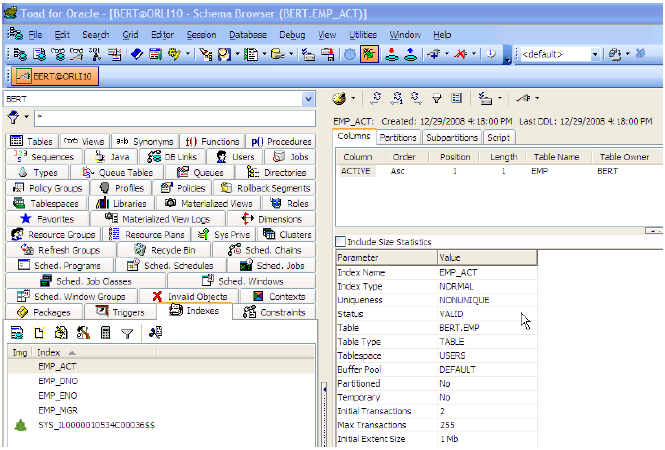
\includegraphics[width=\textwidth]{./figures/GUIoverload.png}
		}
	\end{column}
\end{columns}

\end{frame}


\begin{frame}
\frametitle{R Studio}

	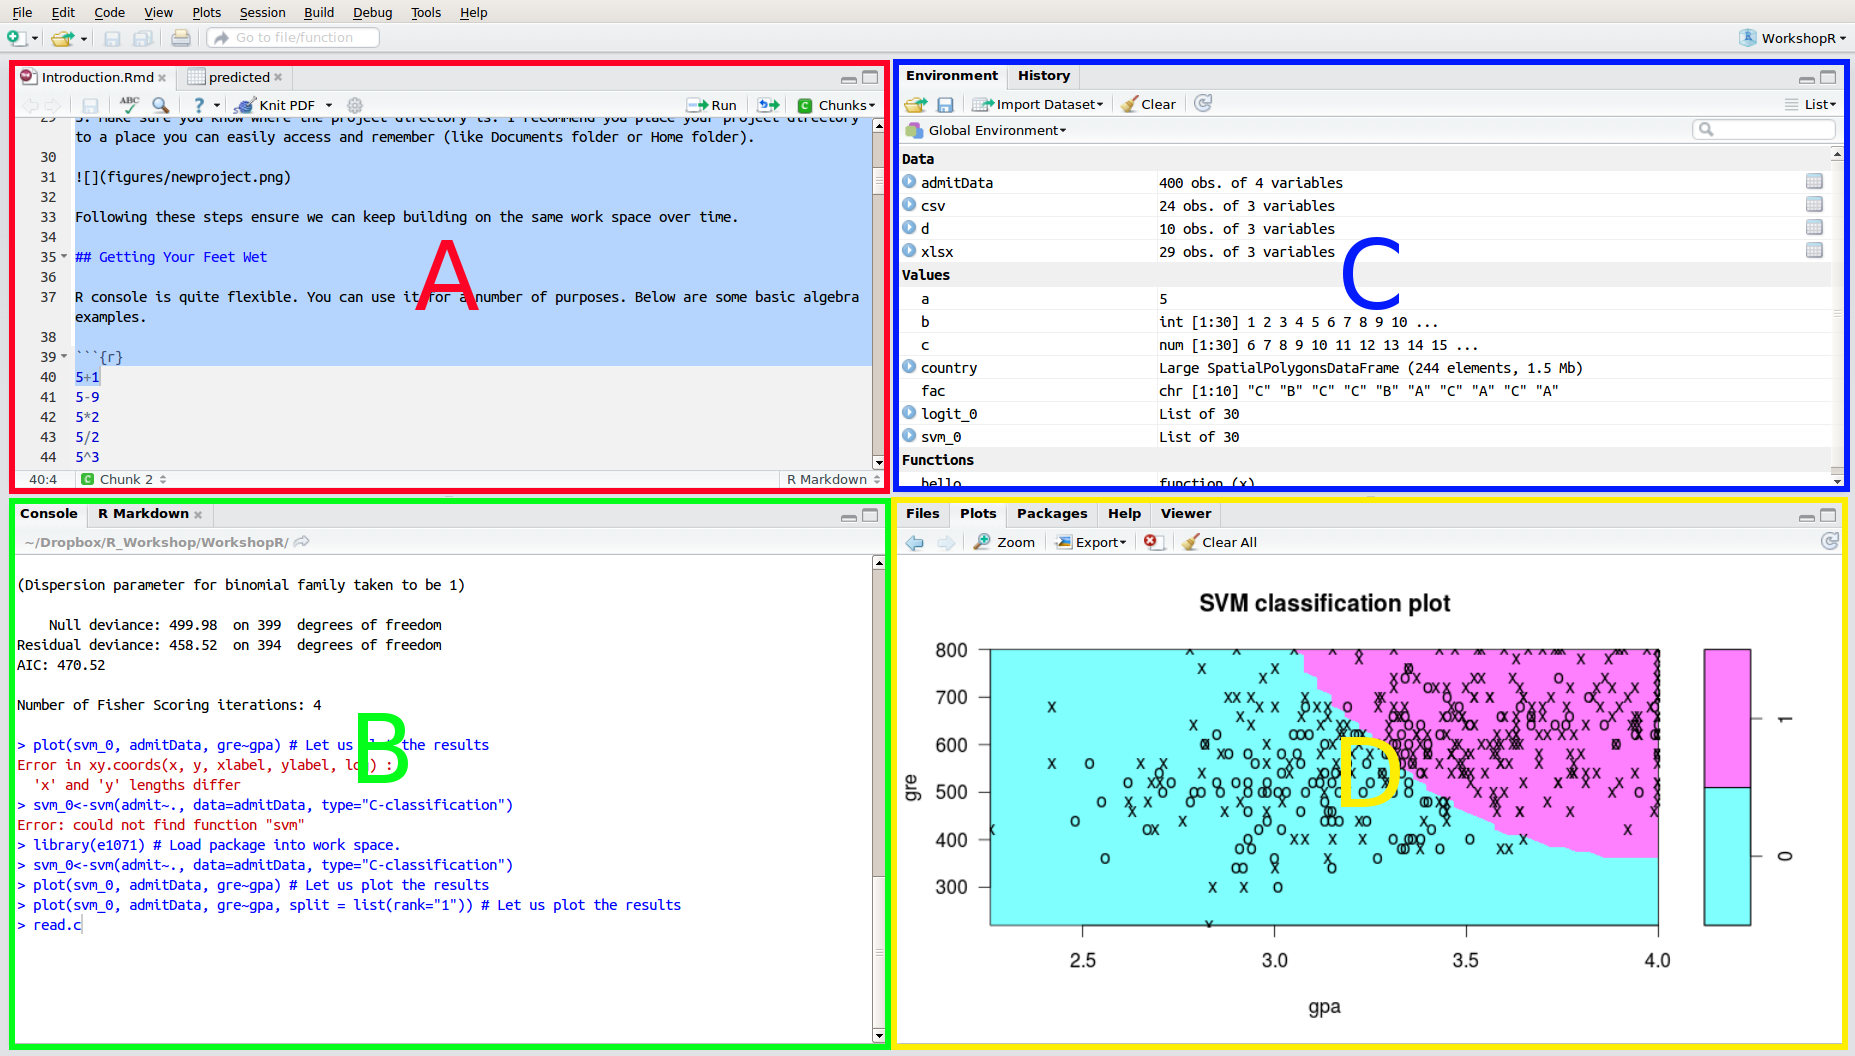
\includegraphics[width=\textwidth]{./figures/studio.png}

\end{frame}

\begin{frame}
\frametitle{New Project}
\vfill
File > New Project
\vfill
Empty Directory > Empty Project > Directory Name: Workshop
\vfill
\end{frame}


\begin{frame}[fragile, allowframebreaks]
\frametitle{R as a Calculator}

\begin{knitrout}\scriptsize
\definecolor{shadecolor}{rgb}{0.969, 0.969, 0.969}\color{fgcolor}\begin{kframe}
\begin{alltt}
\hlcom{# Arithmetics}
\hlnum{2} \hlopt{+} \hlnum{2}
\end{alltt}
\begin{verbatim}
## [1] 4
\end{verbatim}
\begin{alltt}
\hlnum{2} \hlopt{*} \hlnum{3}
\end{alltt}
\begin{verbatim}
## [1] 6
\end{verbatim}
\begin{alltt}
\hlnum{2}\hlopt{^}\hlnum{3}
\end{alltt}
\begin{verbatim}
## [1] 8
\end{verbatim}
\begin{alltt}
\hlkwd{log}\hlstd{(}\hlnum{100}\hlstd{,} \hlnum{10}\hlstd{)}
\end{alltt}
\begin{verbatim}
## [1] 2
\end{verbatim}
\end{kframe}
\end{knitrout}

\begin{knitrout}\scriptsize
\definecolor{shadecolor}{rgb}{0.969, 0.969, 0.969}\color{fgcolor}\begin{kframe}
\begin{alltt}
\hlcom{# Logic}
\hlnum{1} \hlopt{==} \hlnum{2}
\end{alltt}
\begin{verbatim}
## [1] FALSE
\end{verbatim}
\begin{alltt}
\hlnum{1} \hlopt{!=} \hlnum{2}
\end{alltt}
\begin{verbatim}
## [1] TRUE
\end{verbatim}
\begin{alltt}
\hlnum{2} \hlopt{<} \hlnum{3}
\end{alltt}
\begin{verbatim}
## [1] TRUE
\end{verbatim}
\end{kframe}
\end{knitrout}

\end{frame}

\begin{frame}[fragile, allowframebreaks]
\frametitle{Variables}

\begin{knitrout}\scriptsize
\definecolor{shadecolor}{rgb}{0.969, 0.969, 0.969}\color{fgcolor}\begin{kframe}
\begin{alltt}
\hlstd{A} \hlkwb{<-} \hlnum{2}

\hlstd{A}
\end{alltt}
\begin{verbatim}
## [1] 2
\end{verbatim}
\begin{alltt}
\hlcom{# a # Case sensitive}

\hlstr{"A"} \hlopt{!=} \hlstr{"a"}  \hlcom{# Explanation}
\end{alltt}
\begin{verbatim}
## [1] TRUE
\end{verbatim}
\begin{alltt}
\hlstd{B} \hlkwb{<-} \hlnum{7}

\hlstd{A} \hlopt{+} \hlstd{B}
\end{alltt}
\begin{verbatim}
## [1] 9
\end{verbatim}
\end{kframe}
\end{knitrout}

\begin{knitrout}\scriptsize
\definecolor{shadecolor}{rgb}{0.969, 0.969, 0.969}\color{fgcolor}\begin{kframe}
\begin{alltt}
\hlstd{C} \hlkwb{<-} \hlkwd{c}\hlstd{(}\hlnum{1}\hlstd{,} \hlnum{3}\hlstd{,} \hlnum{7}\hlstd{,} \hlnum{9}\hlstd{)}  \hlcom{# A list can be in a variable}

\hlstd{C}
\end{alltt}
\begin{verbatim}
## [1] 1 3 7 9
\end{verbatim}
\begin{alltt}
\hlstd{C} \hlopt{+} \hlstd{A}
\end{alltt}
\begin{verbatim}
## [1]  3  5  9 11
\end{verbatim}
\begin{alltt}
\hlstd{C} \hlopt{*} \hlstd{A}
\end{alltt}
\begin{verbatim}
## [1]  2  6 14 18
\end{verbatim}
\begin{alltt}
\hlstd{C} \hlopt{<} \hlnum{5}
\end{alltt}
\begin{verbatim}
## [1]  TRUE  TRUE FALSE FALSE
\end{verbatim}
\end{kframe}
\end{knitrout}

\end{frame}



\begin{frame}[fragile, allowframebreaks]
\frametitle{Indexes and Data Frames}

\begin{knitrout}\scriptsize
\definecolor{shadecolor}{rgb}{0.969, 0.969, 0.969}\color{fgcolor}\begin{kframe}
\begin{alltt}
\hlnum{1}\hlopt{:}\hlnum{30}
\end{alltt}
\begin{verbatim}
##  [1]  1  2  3  4  5  6  7  8  9 10 11 12 13 14 15 16 17 18 19 20 21 22 23
## [24] 24 25 26 27 28 29 30
\end{verbatim}
\begin{alltt}
\hlstd{C[}\hlnum{3}\hlstd{]}
\end{alltt}
\begin{verbatim}
## [1] 7
\end{verbatim}
\begin{alltt}
\hlstd{C[}\hlkwd{c}\hlstd{(}\hlnum{2}\hlstd{,} \hlnum{3}\hlstd{)]}
\end{alltt}
\begin{verbatim}
## [1] 3 7
\end{verbatim}
\begin{alltt}
\hlstd{C[}\hlnum{1}\hlopt{:}\hlnum{3}\hlstd{]}
\end{alltt}
\begin{verbatim}
## [1] 1 3 7
\end{verbatim}
\end{kframe}
\end{knitrout}

\begin{knitrout}\scriptsize
\definecolor{shadecolor}{rgb}{0.969, 0.969, 0.969}\color{fgcolor}\begin{kframe}
\begin{alltt}
\hlstd{Countries} \hlkwb{<-} \hlkwd{data.frame}\hlstd{(}\hlkwc{names}\hlstd{=}\hlkwd{c}\hlstd{(}\hlstr{"US"}\hlstd{,}\hlstr{"TR"}\hlstd{,}\hlstr{"DE"}\hlstd{),} \hlkwc{supply}\hlstd{=}\hlkwd{c}\hlstd{(}\hlnum{10}\hlstd{,} \hlnum{8}\hlstd{,} \hlnum{7}\hlstd{),}
                        \hlkwc{those}\hlstd{=}\hlkwd{c}\hlstd{(}\hlnum{TRUE}\hlstd{,} \hlnum{FALSE}\hlstd{,} \hlnum{FALSE}\hlstd{))}

\hlstd{Countries}
\end{alltt}
\begin{verbatim}
##   names supply those
## 1    US     10  TRUE
## 2    TR      8 FALSE
## 3    DE      7 FALSE
\end{verbatim}
\end{kframe}
\end{knitrout}

\begin{knitrout}\scriptsize
\definecolor{shadecolor}{rgb}{0.969, 0.969, 0.969}\color{fgcolor}\begin{kframe}
\begin{alltt}
\hlstd{Countries[}\hlnum{2}\hlstd{, ]}
\end{alltt}
\begin{verbatim}
##   names supply those
## 2    TR      8 FALSE
\end{verbatim}
\begin{alltt}
\hlstd{Countries[,} \hlnum{3}\hlstd{]}
\end{alltt}
\begin{verbatim}
## [1]  TRUE FALSE FALSE
\end{verbatim}
\begin{alltt}
\hlstd{Countries[}\hlnum{2}\hlstd{,} \hlnum{3}\hlstd{]}
\end{alltt}
\begin{verbatim}
## [1] FALSE
\end{verbatim}
\begin{alltt}
\hlstd{Countries[}\hlnum{1}\hlopt{:}\hlnum{2}\hlstd{, ]}
\end{alltt}
\begin{verbatim}
##   names supply those
## 1    US     10  TRUE
## 2    TR      8 FALSE
\end{verbatim}
\end{kframe}
\end{knitrout}

\begin{knitrout}\scriptsize
\definecolor{shadecolor}{rgb}{0.969, 0.969, 0.969}\color{fgcolor}\begin{kframe}
\begin{alltt}
\hlstd{Countries[,} \hlstr{"names"}\hlstd{]}
\end{alltt}
\begin{verbatim}
## [1] US TR DE
## Levels: DE TR US
\end{verbatim}
\begin{alltt}
\hlstd{Countries}\hlopt{$}\hlstd{names}
\end{alltt}
\begin{verbatim}
## [1] US TR DE
## Levels: DE TR US
\end{verbatim}
\begin{alltt}
\hlstd{Countries}\hlopt{$}\hlstd{those}
\end{alltt}
\begin{verbatim}
## [1]  TRUE FALSE FALSE
\end{verbatim}
\end{kframe}
\end{knitrout}

\end{frame}

\begin{frame}
\frametitle{Loops in R}
{\Huge {\color{red} CAUTION!}}
\vfill
R is notoriously inefficient with your classic loops
\vfill

\begin{itemize}
	\item Structure of the Data Frame
	\item Memory Management
\end{itemize}
\vfill
Try to use an apply function instead. 
\vfill
Vectorize your operations.

\end{frame}

\begin{frame}[fragile]
\frametitle{For Loop in R}
\begin{knitrout}\scriptsize
\definecolor{shadecolor}{rgb}{0.969, 0.969, 0.969}\color{fgcolor}\begin{kframe}
\begin{alltt}
\hlkwa{for} \hlstd{(i} \hlkwa{in} \hlnum{1}\hlopt{:}\hlnum{3}\hlstd{)} \hlkwd{print}\hlstd{(i)}
\end{alltt}
\begin{verbatim}
## [1] 1
## [1] 2
## [1] 3
\end{verbatim}
\begin{alltt}
\hlcom{# Iterating through a data frame}
\hlkwa{for} \hlstd{(i} \hlkwa{in} \hlnum{1}\hlopt{:}\hlkwd{nrow}\hlstd{(Countries)) \{}
    \hlkwd{print}\hlstd{(Countries[i, ])}
\hlstd{\}}
\end{alltt}
\begin{verbatim}
##   names supply those
## 1    US     10  TRUE
##   names supply those
## 2    TR      8 FALSE
##   names supply those
## 3    DE      7 FALSE
\end{verbatim}
\end{kframe}
\end{knitrout}

\end{frame}


\begin{frame}[fragile, allowframebreaks]
\frametitle{Functions}



\begin{knitrout}\scriptsize
\definecolor{shadecolor}{rgb}{0.969, 0.969, 0.969}\color{fgcolor}\begin{kframe}
\begin{alltt}
\hlkwd{mean}\hlstd{(C)}  \hlcom{# Takes parameters}
\end{alltt}
\begin{verbatim}
## [1] 5
\end{verbatim}
\begin{alltt}
\hlkwd{mean}\hlstd{(C,} \hlkwc{trim} \hlstd{=} \hlnum{0.1}\hlstd{,} \hlkwc{na.rm} \hlstd{= T)}  \hlcom{# Takes multiple parameters}
\end{alltt}
\begin{verbatim}
## [1] 5
\end{verbatim}
\begin{alltt}
\hlkwd{log}\hlstd{(}\hlkwd{sum}\hlstd{(C)}\hlopt{/}\hlkwd{length}\hlstd{(C))}  \hlcom{# Can be combined}
\end{alltt}
\begin{verbatim}
## [1] 1.609438
\end{verbatim}
\end{kframe}
\end{knitrout}

\begin{knitrout}\scriptsize
\definecolor{shadecolor}{rgb}{0.969, 0.969, 0.969}\color{fgcolor}\begin{kframe}
\begin{alltt}
\hlstd{HelloWorld} \hlkwb{<-} \hlkwa{function}\hlstd{(}\hlkwc{x}\hlstd{,} \hlkwc{y} \hlstd{=} \hlnum{1}\hlstd{) \{}
    \hlkwa{for} \hlstd{(i} \hlkwa{in} \hlnum{1}\hlopt{:}\hlstd{y) \{}
        \hlkwd{print}\hlstd{(}\hlkwd{paste}\hlstd{(}\hlstr{"Hello"}\hlstd{, x))}
    \hlstd{\}}
\hlstd{\}}

\hlkwd{HelloWorld}\hlstd{(}\hlstr{"COB Faculty"}\hlstd{)}
\end{alltt}
\begin{verbatim}
## [1] "Hello COB Faculty"
\end{verbatim}
\begin{alltt}
\hlkwd{HelloWorld}\hlstd{(}\hlstr{"COB Faculty"}\hlstd{,} \hlnum{2}\hlstd{)}
\end{alltt}
\begin{verbatim}
## [1] "Hello COB Faculty"
## [1] "Hello COB Faculty"
\end{verbatim}
\end{kframe}
\end{knitrout}

\begin{knitrout}\scriptsize
\definecolor{shadecolor}{rgb}{0.969, 0.969, 0.969}\color{fgcolor}\begin{kframe}
\begin{alltt}
\hlstd{HelloWorld}  \hlcom{# Review the source code}
\end{alltt}
\begin{verbatim}
## function(x, y = 1) {
##     for (i in 1:y) {
##         print(paste("Hello", x))
##     }
## }
## <bytecode: 0x143953e8>
\end{verbatim}
\begin{alltt}
\hlstd{ls}
\end{alltt}
\begin{verbatim}
## function (name, pos = -1L, envir = as.environment(pos), all.names = FALSE, 
##     pattern, sorted = TRUE) 
## {
##     if (!missing(name)) {
##         pos <- tryCatch(name, error = function(e) e)
##         if (inherits(pos, "error")) {
##             name <- substitute(name)
##             if (!is.character(name)) 
##                 name <- deparse(name)
##             warning(gettextf("%s converted to character string", 
##                 sQuote(name)), domain = NA)
##             pos <- name
##         }
##     }
##     all.names <- .Internal(ls(envir, all.names, sorted))
##     if (!missing(pattern)) {
##         if ((ll <- length(grep("[", pattern, fixed = TRUE))) && 
##             ll != length(grep("]", pattern, fixed = TRUE))) {
##             if (pattern == "[") {
##                 pattern <- "\\["
##                 warning("replaced regular expression pattern '[' by  '\\\\['")
##             }
##             else if (length(grep("[^\\\\]\\[<-", pattern))) {
##                 pattern <- sub("\\[<-", "\\\\\\[<-", pattern)
##                 warning("replaced '[<-' by '\\\\[<-' in regular expression pattern")
##             }
##         }
##         grep(pattern, all.names, value = TRUE)
##     }
##     else all.names
## }
## <bytecode: 0x28ba5b8>
## <environment: namespace:base>
\end{verbatim}
\end{kframe}
\end{knitrout}
\end{frame}

\begin{frame}[fragile,allowframebreaks]
\frametitle{Commonly Used Functions}
\begin{knitrout}\scriptsize
\definecolor{shadecolor}{rgb}{0.969, 0.969, 0.969}\color{fgcolor}\begin{kframe}
\begin{alltt}
\hlkwd{ls}\hlstd{()}  \hlcom{# Get a list of objects in the workspace}
\end{alltt}
\begin{verbatim}
## [1] "A"          "admitData"  "B"          "C"          "Countries" 
## [6] "HelloWorld" "i"
\end{verbatim}
\begin{alltt}
\hlkwd{ls}\hlstd{(}\hlkwc{pattern} \hlstd{=} \hlstr{"*_0"}\hlstd{)}  \hlcom{# partial match on object search}
\end{alltt}
\begin{verbatim}
## character(0)
\end{verbatim}
\begin{alltt}
\hlkwd{rm}\hlstd{(}\hlstr{"svm_0"}\hlstd{)}  \hlcom{# Remove an object from the workspace}
\end{alltt}


{\ttfamily\noindent\color{warningcolor}{\#\# Warning in rm("{}svm\_0"{}): object 'svm\_0' not found}}\begin{alltt}
\hlcom{# rm(list=ls()) # This would remove everything if ran}
\end{alltt}
\end{kframe}
\end{knitrout}


\begin{knitrout}\scriptsize
\definecolor{shadecolor}{rgb}{0.969, 0.969, 0.969}\color{fgcolor}\begin{kframe}
\begin{alltt}
\hlkwd{mean}\hlstd{(A)}  \hlcom{# Mean}
\end{alltt}
\begin{verbatim}
## [1] 2
\end{verbatim}
\begin{alltt}
\hlkwd{sd}\hlstd{(admitData[,} \hlstr{"gre"}\hlstd{])}  \hlcom{# Standard Deviation}
\end{alltt}
\begin{verbatim}
## [1] 115.5165
\end{verbatim}
\begin{alltt}
\hlcom{# AIC()}
\end{alltt}
\end{kframe}
\end{knitrout}



\begin{knitrout}\scriptsize
\definecolor{shadecolor}{rgb}{0.969, 0.969, 0.969}\color{fgcolor}\begin{kframe}
\begin{alltt}
\hlkwd{str}\hlstd{(Countries)}  \hlcom{# Look at the structure of objects}
\end{alltt}
\begin{verbatim}
## 'data.frame':	3 obs. of  3 variables:
##  $ names : Factor w/ 3 levels "DE","TR","US": 3 2 1
##  $ supply: num  10 8 7
##  $ those : logi  TRUE FALSE FALSE
\end{verbatim}
\begin{alltt}
\hlkwd{summary}\hlstd{(Countries)}  \hlcom{# Get summary of data}
\end{alltt}
\begin{verbatim}
##  names      supply         those        
##  DE:1   Min.   : 7.000   Mode :logical  
##  TR:1   1st Qu.: 7.500   FALSE:2        
##  US:1   Median : 8.000   TRUE :1        
##         Mean   : 8.333                  
##         3rd Qu.: 9.000                  
##         Max.   :10.000
\end{verbatim}
\end{kframe}
\end{knitrout}



\begin{knitrout}\tiny
\definecolor{shadecolor}{rgb}{0.969, 0.969, 0.969}\color{fgcolor}\begin{kframe}
\begin{alltt}
\hlkwd{summary}\hlstd{(logit_1)}  \hlcom{# Get summary of model}
\end{alltt}
\begin{verbatim}
## 
## Call:
## glm(formula = admit ~ gre, family = "binomial", data = admitData)
## 
## Deviance Residuals: 
##     Min       1Q   Median       3Q      Max  
## -1.1623  -0.9052  -0.7547   1.3486   1.9879  
## 
## Coefficients:
##              Estimate Std. Error z value Pr(>|z|)    
## (Intercept) -2.901344   0.606038  -4.787 1.69e-06 ***
## gre          0.003582   0.000986   3.633  0.00028 ***
## ---
## Signif. codes:  0 '***' 0.001 '**' 0.01 '*' 0.05 '.' 0.1 ' ' 1
## 
## (Dispersion parameter for binomial family taken to be 1)
## 
##     Null deviance: 499.98  on 399  degrees of freedom
## Residual deviance: 486.06  on 398  degrees of freedom
## AIC: 490.06
## 
## Number of Fisher Scoring iterations: 4
\end{verbatim}
\end{kframe}
\end{knitrout}

\begin{knitrout}\scriptsize
\definecolor{shadecolor}{rgb}{0.969, 0.969, 0.969}\color{fgcolor}\begin{kframe}
\begin{alltt}
\hlkwd{cor}\hlstd{(admitData[,} \hlnum{1}\hlopt{:}\hlnum{3}\hlstd{])}  \hlcom{# Get correlation matrix}
\end{alltt}
\begin{verbatim}
##           admit       gre       gpa
## admit 1.0000000 0.1844343 0.1782123
## gre   0.1844343 1.0000000 0.3842659
## gpa   0.1782123 0.3842659 1.0000000
\end{verbatim}
\end{kframe}
\end{knitrout}

\end{frame}


\begin{frame}
	\frametitle{Questions}
	\begin{center}
		\vfill
			\resizebox{!}{.75\textheight}{\Huge \color{red} ?}
		\vfill
	\end{center}
\end{frame}


\section{Importing Data}

\begin{frame}
\frametitle{Importing Data}

R allows importing data from a wide variety of sources. \vspace{1em}

\begin{itemize}
\item Comma Separated Values (CSV)
\item Databases
\item Flat files
\item Lesser statistical packages
\item and more
\end{itemize}

\end{frame}

\begin{frame}[fragile]
\frametitle{Importing CSV Files}

CSV has certain advantages that make it popular.

\begin{columns}[T]
	\begin{column}{.5\textwidth}
		\begin{itemize}
		\vspace{1.5em}
		\item Compatibility
		\item Flexibility
		\item Simplicity
		\end{itemize}
	\end{column}
	\begin{column}{.5\textwidth}
		\begin{alertblock}{Sample}
		{\scriptsize
		"iso2", "Supply", "Those" \\
		"AU",         20,       0 \\
		"TR",         80,       1 \\
		"US",        100,       0 \\
		"GB",         50,       0 \\
		"DE",         70,       0 \\
		}
		\end{alertblock}
	\end{column}
\end{columns}

\vspace{1em}
We use read.csv() or read.csv2() commands to import the csv files.

\begin{knitrout}\scriptsize
\definecolor{shadecolor}{rgb}{0.969, 0.969, 0.969}\color{fgcolor}\begin{kframe}
\begin{alltt}
\hlstd{saveData} \hlkwb{<-} \hlkwd{read.csv}\hlstd{(}\hlstr{"PathToCSV"}\hlstd{,} \hlkwc{header} \hlstd{=} \hlnum{TRUE}\hlstd{,} \hlkwc{sep} \hlstd{=} \hlstr{","}\hlstd{,} \hlkwc{quote} \hlstd{=} \hlstr{"\textbackslash{}""}\hlstd{)}
\end{alltt}
\end{kframe}
\end{knitrout}

\end{frame}


\begin{frame}[fragile]
\frametitle{Working with Excel Files}

Much like CSV, except it lacks the simplicity, flexibility, and compatibility of CSV.

\begin{knitrout}\scriptsize
\definecolor{shadecolor}{rgb}{0.969, 0.969, 0.969}\color{fgcolor}\begin{kframe}
\begin{alltt}
\hlcom{# Load the necessary library}
\hlkwd{library}\hlstd{(xlsx)}
\hlcom{# Read in the data from excel file}
\hlstd{xlsx} \hlkwb{<-} \hlkwd{read.xlsx}\hlstd{(}\hlstr{"country.xlsx"}\hlstd{,} \hlkwc{sheetIndex} \hlstd{=} \hlnum{1}\hlstd{)}
\end{alltt}
\end{kframe}
\end{knitrout}

\end{frame}


\begin{frame}[c]
\frametitle{Working with Databases}

\begin{columns}[T]
	\begin{column}{.5\textwidth}
		No speed advantage.\vspace{1em}

		Data larger than memory.\vspace{1em}

		Working with databases:
		\begin{itemize}
			\item Work in the database.
			\item Import data from database.
		\end{itemize}
		\vfill
	\end{column}

	\begin{column}{.5\textwidth}
		
\includegraphics[width=.8\textwidth]{./figures/Database.png}
	\end{column}

\end{columns}

\end{frame}


\begin{frame}[fragile]
\frametitle{Working with Databases}

\begin{knitrout}\scriptsize
\definecolor{shadecolor}{rgb}{0.969, 0.969, 0.969}\color{fgcolor}\begin{kframe}
\begin{alltt}
\hlcom{# Load the necessary library}
\hlkwd{library}\hlstd{(RMySQL)}
\hlcom{# Establish connection to the database.}
\hlstd{channel} \hlkwb{<-} \hlkwd{dbConnect}\hlstd{(}\hlkwd{MySQL}\hlstd{(),} \hlkwc{user} \hlstd{=} \hlstr{"uname"}\hlstd{,} \hlkwc{password} \hlstd{=} \hlstr{"pwd"}\hlstd{,} \hlkwc{host} \hlstd{=} \hlstr{"127.0.01"}\hlstd{,}
    \hlkwc{dbname} \hlstd{=} \hlstr{"exampledata"}\hlstd{)}
\hlcom{# Send query and save results in R workspace}
\hlstd{sql} \hlkwb{<-} \hlkwd{dbGetQuery}\hlstd{(channel,} \hlstr{"SELECT * FROM table;"}\hlstd{)}
\end{alltt}
\end{kframe}
\end{knitrout}

\end{frame}

\begin{frame}
\frametitle{Lesser Statistical Packages :P}
\begin{columns}[T]
	\begin{column}{.5\textwidth}
		\vspace{1em}
		Foreign Package\vspace{1em}

		Newer file formats\vspace{1em}
		\begin{itemize}
			\item sas7bdat
			\item readstata13
		\end{itemize}
	\end{column}
	\begin{column}{.5\textwidth}
		
\includegraphics[width=.8\textwidth]{./figures/lesser.png}
	\end{column}
\end{columns}


\end{frame}


\begin{frame}
	\frametitle{Questions}
	\begin{center}
		\vfill
			\resizebox{!}{.75\textheight}{\color{red} ?}
		\vfill
	\end{center}
\end{frame}


\section{Packages}

\begin{frame}
\frametitle{Packages: Source of R's Power}

\begin{columns}[c]
	\begin{column}{.5\textwidth}
		Encountered already \vspace{1em}

		Make R extendible \vspace{1em}

		Like libraries \vspace{1em}

		Collection of:
		\begin{itemize}
			\item functions
			\item documentation
			\item data files
		\end{itemize}

	\end{column}
	\begin{column}{.5\textwidth}
		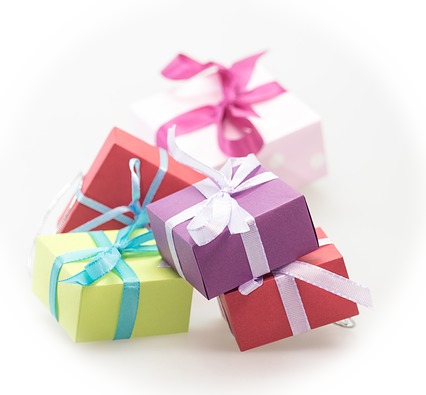
\includegraphics[width=\textwidth]{figures/packages.png}
	\end{column}
\end{columns}

\end{frame}


\begin{frame}
\frametitle{Gifts from the Community}

\begin{columns}[c]
	\begin{column}{.5\textwidth}
		Currently over 13000 packages \vspace{1em}

		for
		\begin{itemize}
			\item Statistical Modeling
			\item Machine Learning
			\item Data Manipulation
			\item Visualization
			\item \ldots
		\end{itemize}

		from
		\begin{itemize}
			\item Economics
			\item Computer Science
			\item Statistics
			\item Medicine
			\item \ldots
		\end{itemize}

	\end{column}
	\begin{column}{.5\textwidth}
		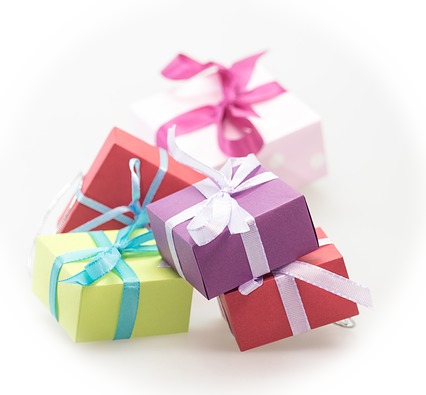
\includegraphics[width=\textwidth]{figures/packages.png}
	\end{column}
\end{columns}

\end{frame}

\begin{frame}
\frametitle{Great but Where are My Gifts?}
\vfill

{\Huge Comprehensive R Archive Network (CRAN)}

\vfill

A Group of FTP and HTML servers hosting R packages.

\vfill

R has built in package management facilities.

\vfill

Most of these can be achieved through the R Studio GUI. (Area D, packages pane)

\vfill

\end{frame}


\begin{frame}[fragile]
\frametitle{Package Management}

\begin{knitrout}\scriptsize
\definecolor{shadecolor}{rgb}{0.969, 0.969, 0.969}\color{fgcolor}\begin{kframe}
\begin{alltt}
\hlcom{# Installing a package}
\hlkwd{install.packages}\hlstd{(}\hlstr{"e1071"}\hlstd{)}  \hlcom{# Notice the quotes around package name}
\hlcom{# Loading package into memory}
\hlkwd{library}\hlstd{(e1071)}  \hlcom{# Notice the lack of quotes}
\hlcom{# Unload package}
\hlkwd{detach}\hlstd{(}\hlstr{"package:e1071"}\hlstd{,} \hlkwc{unload} \hlstd{=} \hlnum{TRUE}\hlstd{)}  \hlcom{# Notice the package: prepended}

\hlcom{# Get the list of packages loaded}
\hlstd{(}\hlkwd{.packages}\hlstd{())}
\hlcom{# Get list of all installed packages (output omitted)}
\hlkwd{.packages}\hlstd{(}\hlkwc{all.available} \hlstd{= T)}
\end{alltt}
\end{kframe}
\end{knitrout}
\end{frame}


\begin{frame}[fragile]
\frametitle{How to Find Packages}

If you want to search a certain word in installed packages' documentation, you can always use ?? or help.search()

\begin{knitrout}\scriptsize
\definecolor{shadecolor}{rgb}{0.969, 0.969, 0.969}\color{fgcolor}\begin{kframe}
\begin{alltt}
\hlopt{??}\hlstd{mixed}
\hlkwd{help.search}\hlstd{(}\hlstr{"mixed model"}\hlstd{)}
\end{alltt}
\end{kframe}
\end{knitrout}

Internet searches are a bit problematic as R can be a bit ambiguous until Google learns you are interested in the statistical computing environment.
\vfill

\href{https://cran.r-project.org/web/packages/}{Comprehensive R Archive Network (CRAN)}
\vfill

\href{https://r-forge.r-project.org/}{R Forge}
\vfill

\href{http://search.r-project.org}{R site search} also available with command RSiteSearch()
\vfill
\href{http://rseek.org/}{R seek}

\end{frame}

\begin{frame}
\frametitle{Commonly Used Packages: Data Manipulation}

\textbf{data.tables} Replaces traditional data.frame. 
\begin{itemize}
	\item Faster access/write
	\item Improved selection 
	\item Improved subsetting 
	\item Improved aggregation 
\end{itemize}

Not a drop-in replacement as it breaks compatibility in some cases.

\vspace{1em}

\textbf{ddplyr}

Additional functionality for:
\begin{itemize}
	\item selection
	\item filtering
	\item aggregation
\end{itemize}

Provides efficient back-end data structures to speed things up. 

Works with databases as well.

\end{frame}

\begin{frame}
\frametitle{Commonly Used Packages: Statistics}

Multiple Regression: Stats package, lm() (loaded by default) \vfill

Generalized Linear Models: Stats package, glm() \vfill

Traditional Econometric Models: plm package \vfill

Mixed Modeling: nlme and lme4 packages \vfill

\end{frame}


\begin{frame}
\frametitle{Commonly Used Packages: Machine Learning}

Most probably all you need is caret package. \vfill

Caret package is a wrapper for a host of classification and regression model training functions. It eases visualizations, data manipulation, and analytics among others. \href{http://topepo.github.io/caret/modelList.html}{It currently supports over 150 types of models.}\vfill 

If you insist on using individual packages:

Classifiers: class package 

Support Vector Machines: kernlab, e1071 packages 

Clustering: Base package (kmeans(), hclust()), mclust package 

Neural Networks: neuralnet package.
\vfill

\end{frame}


\begin{frame}
	\frametitle{Questions}
	\begin{center}
		\vfill
			\resizebox{!}{.75\textheight}{\Huge \color{red} ?}
		\vfill
	\end{center}
\end{frame}

\section{Sample Analysis and Visualizations}


\subsection{Descriptive Visualizations}

\begin{frame}
\frametitle{Motor Trends Dataset}

\href{http://www.jstor.org/stable/2530428}{We will use 1974 Motor Trend dataset. It has 32 observations and 11 variables.} \vfill

\begin{columns}[T]
	\begin{column}{.5\textwidth}
		\begin{itemize}
			\item mpg: Miles per gallon
			\item cyl: Number of cylinders
			\item disp: Displacement
			\item hp: Horse Power
			\item drat: Rear axle ratio
			\item wt: Weight
		\end{itemize}
	\end{column}

	\begin{column}{.5\textwidth}
		\begin{itemize}
			\item qsec: quarter mile time
			\item vs: V - S 
			\item am: 0 automatic, 1 manual
			\item gear: Gears
			\item carb: Number of carburetors
		\end{itemize}
	\end{column}
\end{columns}
\vfill

\end{frame}


\begin{frame}[fragile,allowframebreaks]
\frametitle{Motor Trends Dataset}

\begin{knitrout}\tiny
\definecolor{shadecolor}{rgb}{0.969, 0.969, 0.969}\color{fgcolor}\begin{kframe}
\begin{alltt}
\hlkwd{summary}\hlstd{(mtcars)}
\end{alltt}
\begin{verbatim}
##       mpg             cyl             disp             hp       
##  Min.   :10.40   Min.   :4.000   Min.   : 71.1   Min.   : 52.0  
##  1st Qu.:15.43   1st Qu.:4.000   1st Qu.:120.8   1st Qu.: 96.5  
##  Median :19.20   Median :6.000   Median :196.3   Median :123.0  
##  Mean   :20.09   Mean   :6.188   Mean   :230.7   Mean   :146.7  
##  3rd Qu.:22.80   3rd Qu.:8.000   3rd Qu.:326.0   3rd Qu.:180.0  
##  Max.   :33.90   Max.   :8.000   Max.   :472.0   Max.   :335.0  
##       drat             wt             qsec             vs        
##  Min.   :2.760   Min.   :1.513   Min.   :14.50   Min.   :0.0000  
##  1st Qu.:3.080   1st Qu.:2.581   1st Qu.:16.89   1st Qu.:0.0000  
##  Median :3.695   Median :3.325   Median :17.71   Median :0.0000  
##  Mean   :3.597   Mean   :3.217   Mean   :17.85   Mean   :0.4375  
##  3rd Qu.:3.920   3rd Qu.:3.610   3rd Qu.:18.90   3rd Qu.:1.0000  
##  Max.   :4.930   Max.   :5.424   Max.   :22.90   Max.   :1.0000  
##        am              gear            carb      
##  Min.   :0.0000   Min.   :3.000   Min.   :1.000  
##  1st Qu.:0.0000   1st Qu.:3.000   1st Qu.:2.000  
##  Median :0.0000   Median :4.000   Median :2.000  
##  Mean   :0.4062   Mean   :3.688   Mean   :2.812  
##  3rd Qu.:1.0000   3rd Qu.:4.000   3rd Qu.:4.000  
##  Max.   :1.0000   Max.   :5.000   Max.   :8.000
\end{verbatim}
\end{kframe}
\end{knitrout}

\begin{knitrout}\tiny
\definecolor{shadecolor}{rgb}{0.969, 0.969, 0.969}\color{fgcolor}\begin{kframe}
\begin{alltt}
\hlkwd{pairs}\hlstd{(mtcars[,} \hlkwd{c}\hlstd{(}\hlstr{"mpg"}\hlstd{,} \hlstr{"hp"}\hlstd{,} \hlstr{"am"}\hlstd{,} \hlstr{"cyl"}\hlstd{)])}  \hlcom{# Visualize Correlations}
\end{alltt}
\end{kframe}

{\centering \includegraphics[width=.54\linewidth]{figures/beamer-mtcarspairs-1} 

}



\end{knitrout}
\end{frame}


\begin{frame}[fragile, allowframebreaks]
\frametitle{Histograms}

\begin{knitrout}\scriptsize
\definecolor{shadecolor}{rgb}{0.969, 0.969, 0.969}\color{fgcolor}\begin{kframe}
\begin{alltt}
\hlkwd{data}\hlstd{(mtcars)}  \hlcom{# Load the Dataset}
\hlkwd{library}\hlstd{(ggplot2)}  \hlcom{# Load the ggplot package}
\hlcom{# Nr of cars by number of gears}
\hlkwd{qplot}\hlstd{(}\hlkwd{factor}\hlstd{(gear),} \hlkwc{data} \hlstd{= mtcars,} \hlkwc{geom} \hlstd{=} \hlstr{"bar"}\hlstd{)}
\end{alltt}
\end{kframe}

{\centering \includegraphics[width=.7\linewidth]{figures/beamer-bar0-1} 

}



\end{knitrout}

\begin{knitrout}\scriptsize
\definecolor{shadecolor}{rgb}{0.969, 0.969, 0.969}\color{fgcolor}\begin{kframe}
\begin{alltt}
\hlcom{# If we are interested in a third categorical variable vs:}
\hlkwd{qplot}\hlstd{(}\hlkwd{factor}\hlstd{(gear),} \hlkwc{data}\hlstd{=mtcars,} \hlkwc{geom}\hlstd{=}\hlstr{"bar"}\hlstd{,} \hlkwc{fill}\hlstd{=}\hlkwd{factor}\hlstd{(am))} \hlopt{+}
\hlkwd{ggtitle}\hlstd{(}\hlstr{'Nice Histogram'}\hlstd{)} \hlcom{# This is how you add a title}
\end{alltt}
\end{kframe}

{\centering \includegraphics[width=.7\linewidth]{figures/beamer-bar1-1} 

}



\end{knitrout}
\end{frame}

\begin{frame}[fragile, allowframebreaks]
\frametitle{Scatter Plots}

\begin{knitrout}\scriptsize
\definecolor{shadecolor}{rgb}{0.969, 0.969, 0.969}\color{fgcolor}\begin{kframe}
\begin{alltt}
\hlcom{# Two continuous variables}
\hlkwd{qplot}\hlstd{(hp, mpg,} \hlkwc{data} \hlstd{= mtcars,} \hlkwc{color} \hlstd{=} \hlkwd{factor}\hlstd{(cyl))}
\end{alltt}
\end{kframe}

{\centering \includegraphics[width=.7\linewidth]{figures/beamer-scatter0-1} 

}



\end{knitrout}

\begin{knitrout}\scriptsize
\definecolor{shadecolor}{rgb}{0.969, 0.969, 0.969}\color{fgcolor}\begin{kframe}
\begin{alltt}
\hlcom{# Add two more variables represented by color and size of points}
\hlkwd{qplot}\hlstd{(hp, mpg,} \hlkwc{data} \hlstd{= mtcars,} \hlkwc{color} \hlstd{=} \hlkwd{factor}\hlstd{(cyl),} \hlkwc{size} \hlstd{= disp,} \hlkwc{alpha} \hlstd{=} \hlnum{0.09}\hlstd{)}
\end{alltt}
\end{kframe}

{\centering \includegraphics[width=.7\linewidth]{figures/beamer-scatter1-1} 

}



\end{knitrout}


\end{frame}

\begin{frame}[fragile,allowframebreaks]
\frametitle{Bar Charts}

\begin{knitrout}\scriptsize
\definecolor{shadecolor}{rgb}{0.969, 0.969, 0.969}\color{fgcolor}\begin{kframe}
\begin{alltt}
\hlkwd{ggplot}\hlstd{(mtcars,} \hlkwd{aes}\hlstd{(}\hlkwc{x} \hlstd{=} \hlkwd{factor}\hlstd{(gear),} \hlkwc{y} \hlstd{= mpg,} \hlkwc{fill} \hlstd{=} \hlkwd{factor}\hlstd{(vs)),} \hlkwc{color} \hlstd{=} \hlkwd{factor}\hlstd{(vs))} \hlopt{+}
    \hlkwd{stat_summary}\hlstd{(}\hlkwc{fun.y} \hlstd{= mean,} \hlkwc{position} \hlstd{=} \hlkwd{position_dodge}\hlstd{(),} \hlkwc{geom} \hlstd{=} \hlstr{"bar"}\hlstd{)}
\end{alltt}
\end{kframe}

{\centering \includegraphics[width=.7\linewidth]{figures/beamer-bar2-1} 

}



\end{knitrout}

\end{frame}


% Linear Regression
\subsection{Modeling}

\begin{frame}
\frametitle{Modeling}

Developing a mathematical explanation for real life phenomena.\vfill

Useful in predicting outcomes (Y), and/or explaining the role of drivers (X).\vfill

Y = Outcome Variable, Dependent Variable\ldots\vfill

X = Predictor, Independent variable\ldots\vfill

\end{frame}


\begin{frame}
\frametitle{Formula Interface}

Pay close attention to how we specify the model. \vfill

\begin{alertblock}{R Model}
		Y $\sim x_1 + x_2$
\end{alertblock}
\vfill

This basic structure will remain constant across many R packages.\vfill 

\end{frame}


\begin{frame}
\frametitle{Nifty Tricks with Formula Interface}

If you have lots of variables use the shortcut `.'.

\hspace{4em} mpg $\sim$ . \vfill

You can do transformations on the fly, no need to create variables.

\hspace{4em} log(mpg + 1) $\sim$ .\vfill

Dummy variables.

\hspace{4em} log(mpg + 1) $\sim$ factor(gears) \vfill

\end{frame}


\begin{frame}
\frametitle{Regression}

Y is continuous.\vfill

Prediction.\vfill

Explanation.\vfill

Linearity, Homoscedasticity, Normality, No Multicollinearity

\end{frame}

\begin{frame}[fragile,allowframebreaks]
\frametitle{Regression}

Regression visualized.

\begin{knitrout}\scriptsize
\definecolor{shadecolor}{rgb}{0.969, 0.969, 0.969}\color{fgcolor}\begin{kframe}
\begin{alltt}
\hlkwd{ggplot}\hlstd{(mtcars,} \hlkwd{aes}\hlstd{(}\hlkwc{x} \hlstd{= hp,} \hlkwc{y} \hlstd{= mpg))} \hlopt{+} \hlkwd{geom_point}\hlstd{()} \hlopt{+} \hlcom{# Add a regression line}
\hlkwd{geom_smooth}\hlstd{(}\hlkwc{method} \hlstd{= lm)}
\end{alltt}
\end{kframe}

{\centering \includegraphics[width=.6\linewidth]{figures/beamer-reg1-1} 

}



\end{knitrout}


\end{frame}



\begin{frame}
\frametitle{Multiple Regression Example}

We will keep using motor trends data set.\vfill

\begin{alertblock}{Formula}
	\[
		Y = \beta_0 + \beta_1 x_1 + \beta_2 x_2 + \epsilon
	\]
\end{alertblock}
\vfill
\begin{alertblock}{R Model}
    \[
		Y \sim x_1 + x_2
	\]
\end{alertblock}
\vfill


\end{frame}


\begin{frame}[fragile,allowframebreaks]
\frametitle{Regression}


\begin{knitrout}\tiny
\definecolor{shadecolor}{rgb}{0.969, 0.969, 0.969}\color{fgcolor}\begin{kframe}
\begin{alltt}
\hlcom{# Let us estimate gas milage}
\hlstd{reg_0} \hlkwb{<-} \hlkwd{lm}\hlstd{(mpg} \hlopt{~} \hlstd{hp} \hlopt{+} \hlstd{cyl} \hlopt{+} \hlstd{am, mtcars)}
\hlkwd{summary}\hlstd{(reg_0)}
\end{alltt}
\begin{verbatim}
## 
## Call:
## lm(formula = mpg ~ hp + cyl + am, data = mtcars)
## 
## Residuals:
##    Min     1Q Median     3Q    Max 
## -4.864 -1.811 -0.158  1.492  6.013 
## 
## Coefficients:
##             Estimate Std. Error t value Pr(>|t|)    
## (Intercept) 30.88834    2.78422  11.094 9.27e-12 ***
## hp          -0.03688    0.01452  -2.540  0.01693 *  
## cyl         -1.12721    0.63417  -1.777  0.08636 .  
## am           3.90428    1.29659   3.011  0.00546 ** 
## ---
## Signif. codes:  0 '***' 0.001 '**' 0.01 '*' 0.05 '.' 0.1 ' ' 1
## 
## Residual standard error: 2.807 on 28 degrees of freedom
## Multiple R-squared:  0.8041,	Adjusted R-squared:  0.7831 
## F-statistic: 38.32 on 3 and 28 DF,  p-value: 4.791e-10
\end{verbatim}
\end{kframe}
\end{knitrout}

\begin{knitrout}\tiny
\definecolor{shadecolor}{rgb}{0.969, 0.969, 0.969}\color{fgcolor}\begin{kframe}
\begin{alltt}
\hlcom{## Diagnostics}
\hlkwd{library}\hlstd{(car)}
\hlcom{# Multicollienarity (vif>10 indicates MC)}
\hlkwd{vif}\hlstd{(reg_0)}
\end{alltt}
\begin{verbatim}
##       hp      cyl       am 
## 3.900138 5.048209 1.647399
\end{verbatim}
\begin{alltt}
\hlcom{# Normality (p<0.05 indicates NN)}
\hlkwd{shapiro.test}\hlstd{(reg_0}\hlopt{$}\hlstd{residuals)}
\end{alltt}
\begin{verbatim}
## 
## 	Shapiro-Wilk normality test
## 
## data:  reg_0$residuals
## W = 0.98366, p-value = 0.8961
\end{verbatim}
\begin{alltt}
\hlcom{# Homoscedasticity (p<0.05 indicates Heteroscedasticity)}
\hlkwd{ncvTest}\hlstd{(reg_0)}
\end{alltt}
\begin{verbatim}
## Non-constant Variance Score Test 
## Variance formula: ~ fitted.values 
## Chisquare = 3.744471    Df = 1     p = 0.05298249
\end{verbatim}
\end{kframe}
\end{knitrout}

\begin{knitrout}\scriptsize
\definecolor{shadecolor}{rgb}{0.969, 0.969, 0.969}\color{fgcolor}\begin{kframe}
\begin{alltt}
\hlcom{# Access Fitted Values View first 3 predictions}
\hlstd{reg_0}\hlopt{$}\hlstd{fitted.values[}\hlnum{1}\hlopt{:}\hlnum{3}\hlstd{]}
\end{alltt}
\begin{verbatim}
##     Mazda RX4 Mazda RX4 Wag    Datsun 710 
##      23.97302      23.97302      26.85433
\end{verbatim}
\end{kframe}
\end{knitrout}

\begin{knitrout}\scriptsize
\definecolor{shadecolor}{rgb}{0.969, 0.969, 0.969}\color{fgcolor}\begin{kframe}
\begin{alltt}
\hlcom{# PREDICTING NEW DATA BASED ON MODEL}
\hlstd{newCar} \hlkwb{<-} \hlstd{mtcars[}\hlnum{3}\hlstd{, ]}  \hlcom{# 3rd observation is Datsun 710}
\hlstd{newCar}\hlopt{$}\hlstd{am} \hlkwb{<-} \hlnum{0}  \hlcom{# What if it was automatic?}
\hlstd{reg_0}\hlopt{$}\hlstd{fitted.values[}\hlnum{3}\hlstd{]}  \hlcom{# Previous estimate}
\end{alltt}
\begin{verbatim}
## Datsun 710 
##   26.85433
\end{verbatim}
\begin{alltt}
\hlkwd{predict}\hlstd{(reg_0,} \hlkwc{newdata} \hlstd{= newCar)}  \hlcom{# Datsun with automatic transmission}
\end{alltt}
\begin{verbatim}
## Datsun 710 
##   22.95005
\end{verbatim}
\end{kframe}
\end{knitrout}

\begin{knitrout}\scriptsize
\definecolor{shadecolor}{rgb}{0.969, 0.969, 0.969}\color{fgcolor}\begin{kframe}
\begin{alltt}
\hlcom{## Plot the residuals against observation}
\hlkwd{qplot}\hlstd{(}\hlkwc{data}\hlstd{=mtcars,} \hlkwc{x} \hlstd{= mpg,} \hlkwc{y} \hlstd{= reg_0}\hlopt{$}\hlstd{residuals)} \hlopt{+} \hlcom{#$}
        \hlkwd{stat_smooth}\hlstd{(}\hlkwc{method} \hlstd{=} \hlstr{"lm"}\hlstd{,} \hlkwc{col} \hlstd{=} \hlstr{"red"}\hlstd{)}
\end{alltt}
\end{kframe}

{\centering \includegraphics[width=.7\linewidth]{figures/beamer-regplot-1} 

}



\end{knitrout}

\begin{knitrout}\scriptsize
\definecolor{shadecolor}{rgb}{0.969, 0.969, 0.969}\color{fgcolor}\begin{kframe}
\begin{alltt}
\hlcom{## COMPARE MODELS}
\hlstd{reg_1} \hlkwb{<-} \hlkwd{lm}\hlstd{(mpg} \hlopt{~} \hlstd{hp} \hlopt{+} \hlstd{cyl} \hlopt{+} \hlstd{am} \hlopt{+} \hlstd{wt, mtcars)}  \hlcom{# add weight}
\hlkwd{anova}\hlstd{(reg_0, reg_1)}
\end{alltt}
\begin{verbatim}
## Analysis of Variance Table
## 
## Model 1: mpg ~ hp + cyl + am
## Model 2: mpg ~ hp + cyl + am + wt
##   Res.Df    RSS Df Sum of Sq      F   Pr(>F)   
## 1     28 220.55                                
## 2     27 170.00  1    50.555 8.0295 0.008603 **
## ---
## Signif. codes:  0 '***' 0.001 '**' 0.01 '*' 0.05 '.' 0.1 ' ' 1
\end{verbatim}
\begin{alltt}
\hlcom{# AIC of the model}
\hlkwd{AIC}\hlstd{(reg_0)}
\end{alltt}
\begin{verbatim}
## [1] 162.5849
\end{verbatim}
\begin{alltt}
\hlkwd{AIC}\hlstd{(reg_1)}
\end{alltt}
\begin{verbatim}
## [1] 156.2536
\end{verbatim}
\begin{alltt}
\hlcom{# Also the R-square}
\end{alltt}
\end{kframe}
\end{knitrout}

\end{frame}



% Logistic Regression
\begin{frame}
\frametitle{Logistic Regression}

Ordinary least squares regression was great for predicting continuous variables.\vfill

What if we are interested in predicting categories?\vfill

If there are only two categories (binary) logistic regression is a viable alternative.\vfill

Idea is similar to OLS regression. The only difference is we predict a constrained outcome (probability).

\end{frame}


\begin{frame}
\frametitle{Logistic Regression}

Dependent variable will be type (binary). \vfill

It is basically a regression with a binomial link function. \vfill

\begin{alertblock}{Formula}
\[
log \left(\frac{p}{1-p} \right) = \beta_0 + \beta_1 x_1 + \epsilon
\]
\end{alertblock}

\end{frame}


\begin{frame}[fragile,allowframebreaks]
\frametitle{Logit}


\begin{knitrout}\tiny
\definecolor{shadecolor}{rgb}{0.969, 0.969, 0.969}\color{fgcolor}\begin{kframe}
\begin{alltt}
\hlstd{logit_2} \hlkwb{<-} \hlkwd{glm}\hlstd{(am} \hlopt{~} \hlstd{mpg} \hlopt{+} \hlstd{drat} \hlopt{+} \hlstd{cyl,} \hlkwc{data} \hlstd{= mtcars,} \hlkwc{family} \hlstd{=} \hlstr{"binomial"}\hlstd{)}
\hlkwd{summary}\hlstd{(logit_2)}
\end{alltt}
\begin{verbatim}
## 
## Call:
## glm(formula = am ~ mpg + drat + cyl, family = "binomial", data = mtcars)
## 
## Deviance Residuals: 
##      Min        1Q    Median        3Q       Max  
## -1.58367  -0.31020  -0.03757   0.17972   1.75395  
## 
## Coefficients:
##             Estimate Std. Error z value Pr(>|z|)  
## (Intercept) -49.4548    24.1280  -2.050   0.0404 *
## mpg           0.6378     0.4266   1.495   0.1349  
## drat          7.2595     3.2702   2.220   0.0264 *
## cyl           1.6115     1.0801   1.492   0.1357  
## ---
## Signif. codes:  0 '***' 0.001 '**' 0.01 '*' 0.05 '.' 0.1 ' ' 1
## 
## (Dispersion parameter for binomial family taken to be 1)
## 
##     Null deviance: 43.23  on 31  degrees of freedom
## Residual deviance: 17.03  on 28  degrees of freedom
## AIC: 25.03
## 
## Number of Fisher Scoring iterations: 7
\end{verbatim}
\end{kframe}
\end{knitrout}

\begin{knitrout}\scriptsize
\definecolor{shadecolor}{rgb}{0.969, 0.969, 0.969}\color{fgcolor}\begin{kframe}
\begin{alltt}
\hlcom{# VISUALIZE mpg - Transmission RELATION}
\hlkwd{ggplot}\hlstd{(mtcars,} \hlkwd{aes}\hlstd{(}\hlkwc{x} \hlstd{= mpg,} \hlkwc{y} \hlstd{= am))} \hlopt{+}
        \hlkwd{stat_smooth}\hlstd{(}\hlkwc{method}\hlstd{=}\hlstr{"glm"}\hlstd{,} \hlkwc{family}\hlstd{=}\hlstr{"binomial"}\hlstd{,} \hlkwc{se}\hlstd{=}\hlnum{FALSE}\hlstd{)} \hlcom{#}
\end{alltt}


{\ttfamily\noindent\color{warningcolor}{\#\# Warning: Ignoring unknown parameters: family}}\end{kframe}

{\centering \includegraphics[width=.7\linewidth]{figures/beamer-logitplot2-1} 

}



\end{knitrout}


\begin{knitrout}\scriptsize
\definecolor{shadecolor}{rgb}{0.969, 0.969, 0.969}\color{fgcolor}\begin{kframe}
\begin{alltt}
\hlcom{## VISUALIZE Mpg - Transmission FOR DIFFERENT NUMBERS OF CYLINDERS}

\hlcom{# Create a new dataset with varying number of cylinders and other variables}
\hlcom{# fixed at mean levels.}
\hlstd{mtcars2} \hlkwb{<-} \hlkwd{data.frame}\hlstd{(}\hlkwc{mpg} \hlstd{=} \hlkwd{rep}\hlstd{(}\hlnum{10}\hlopt{:}\hlnum{30}\hlstd{,} \hlnum{3}\hlstd{),} \hlkwc{drat} \hlstd{=} \hlkwd{mean}\hlstd{(mtcars}\hlopt{$}\hlstd{drat),} \hlkwc{disp} \hlstd{=} \hlkwd{mean}\hlstd{(mtcars}\hlopt{$}\hlstd{disp),}
    \hlkwc{cyl} \hlstd{=} \hlkwd{rep}\hlstd{(}\hlkwd{c}\hlstd{(}\hlnum{4}\hlstd{,} \hlnum{6}\hlstd{,} \hlnum{8}\hlstd{),} \hlnum{21}\hlstd{))}
\hlcom{# Predict probability of new data}
\hlstd{mtcars2}\hlopt{$}\hlstd{prob} \hlkwb{<-} \hlkwd{predict}\hlstd{(logit_2,} \hlkwc{newdata} \hlstd{= mtcars2,} \hlkwc{type} \hlstd{=} \hlstr{"response"}\hlstd{)}

\hlcom{# Plot the results}
\hlkwd{ggplot}\hlstd{(mtcars2,} \hlkwd{aes}\hlstd{(}\hlkwc{x} \hlstd{= mpg,} \hlkwc{y} \hlstd{= prob))} \hlopt{+} \hlkwd{geom_line}\hlstd{(}\hlkwd{aes}\hlstd{(}\hlkwc{colour} \hlstd{=} \hlkwd{factor}\hlstd{(cyl)),}
    \hlkwc{size} \hlstd{=} \hlnum{1}\hlstd{)}  \hlcom{# a different color for each category$}
\end{alltt}
\end{kframe}

{\centering \includegraphics[width=.9\linewidth]{figures/beamer-logitplot3-1} 

}



\end{knitrout}

\begin{knitrout}\scriptsize
\definecolor{shadecolor}{rgb}{0.969, 0.969, 0.969}\color{fgcolor}\begin{kframe}
\begin{alltt}
\hlcom{## DIAGNOSTICS}

\hlcom{# Let us compare predicted values to real values}
\hlstd{mtcars}\hlopt{$}\hlstd{prob} \hlkwb{<-} \hlkwd{predict}\hlstd{(logit_2,} \hlkwc{type} \hlstd{=} \hlstr{"response"}\hlstd{)}
\hlcom{# Prevalence of Manual Transmission}
\hlkwd{mean}\hlstd{(mtcars}\hlopt{$}\hlstd{am)}
\end{alltt}
\begin{verbatim}
## [1] 0.40625
\end{verbatim}
\begin{alltt}
\hlcom{# Create predict variable}
\hlstd{mtcars}\hlopt{$}\hlstd{pred} \hlkwb{<-} \hlnum{0}
\hlcom{# If probability is greater than .6 (1-prevalence), set prediction to 1}
\hlstd{mtcars[mtcars}\hlopt{$}\hlstd{prob} \hlopt{>} \hlnum{0.6}\hlstd{,} \hlstr{"pred"}\hlstd{]} \hlkwb{<-} \hlnum{1}
\end{alltt}
\end{kframe}
\end{knitrout}

\begin{knitrout}\scriptsize
\definecolor{shadecolor}{rgb}{0.969, 0.969, 0.969}\color{fgcolor}\begin{kframe}
\begin{alltt}
\hlcom{## ROC CURVE}

\hlcom{# Load the necessary library}
\hlkwd{library}\hlstd{(pROC)}
\hlcom{# Calculate the ROC curve using the predicted probability vs actual values}
\hlstd{logit_2_roc} \hlkwb{<-} \hlkwd{roc}\hlstd{(am} \hlopt{~} \hlstd{prob, mtcars)}
\hlcom{# Plot ROC curve}
\hlkwd{plot}\hlstd{(logit_2_roc)}
\end{alltt}
\end{kframe}

{\centering \includegraphics[width=.5\linewidth]{figures/beamer-logitroc-1} 

}



\end{knitrout}

\begin{knitrout}\tiny
\definecolor{shadecolor}{rgb}{0.969, 0.969, 0.969}\color{fgcolor}\begin{kframe}
\begin{alltt}
\hlkwd{library}\hlstd{(caret)}  \hlcom{# Needed for Confusion Matrix}
\hlkwd{confusionMatrix}\hlstd{(}\hlkwd{table}\hlstd{(mtcars[,} \hlkwd{c}\hlstd{(}\hlstr{"am"}\hlstd{,} \hlstr{"pred"}\hlstd{)]))}
\end{alltt}
\begin{verbatim}
## Confusion Matrix and Statistics
## 
##    pred
## am   0  1
##   0 18  1
##   1  3 10
##                                           
##                Accuracy : 0.875           
##                  95% CI : (0.7101, 0.9649)
##     No Information Rate : 0.6562          
##     P-Value [Acc > NIR] : 0.005004        
##                                           
##                   Kappa : 0.7344          
##  Mcnemar's Test P-Value : 0.617075        
##                                           
##             Sensitivity : 0.8571          
##             Specificity : 0.9091          
##          Pos Pred Value : 0.9474          
##          Neg Pred Value : 0.7692          
##              Prevalence : 0.6562          
##          Detection Rate : 0.5625          
##    Detection Prevalence : 0.5938          
##       Balanced Accuracy : 0.8831          
##                                           
##        'Positive' Class : 0               
## 
\end{verbatim}
\end{kframe}
\end{knitrout}

\end{frame}



\begin{frame}
	\frametitle{Questions}
	\begin{center}
		\vfill
			\resizebox{!}{.75\textheight}{\Huge \color{red} ?}
		\vfill
	\end{center}
\end{frame}

\section{Reporting}

\begin{frame}
\frametitle{Markdown and R Markdown}

Think HTML simplified. \vfill

Add (R) code into it. \vfill

Stir well with knitr \vfill

\end{frame}

\begin{frame}[fragile]
\frametitle{R Markdown Cheat Sheet}

\#   {\Huge \textbf{H1}}

\#\#  {\Large \textbf{H2}}

\#\#\# \textbf{H3} \vfill

*{\textit{Italic}}*

**{\textbf{Bold}}**

***{\textit{ \textbf{Bold Italic}}}*** \vfill

\begin{verbatim}
``` { r, options }
R CODE HERE
```
\end{verbatim}

\end{frame}


\begin{frame}
\frametitle{Professional Looking Documents}

All the documentation of this workshop has been prepared in R Studio. \vfill

Look into the Rmd documents to see how this was done. \vfill

summary() function does not provide the best looking model summaries.
Try the texreg package (do as I say, not as I do).\vfill

Use themes for your plots.

\end{frame}


\begin{frame}
\frametitle{Other Reporting Alternatives}

Sweave: \LaTeX \vfill

Beamer: \LaTeX ~ presentations \vfill

Shiny: Web Applications \vfill

\end{frame}


\begin{frame}
	\frametitle{Questions}
	\begin{center}
		\vfill
			\resizebox{!}{.75\textheight}{\Huge \color{red} ?}
		\vfill
	\end{center}
\end{frame}


\section{Where to Go Next?}

\begin{frame}
\frametitle{Quo Vadis?}

4 hours is not enough! \vfill

RTFM\footnote{Read the Friendly Manual}: Documentation is your friend, read the vignettes and manuals.\vfill

For tutorials: \href{http://www.ats.ucla.edu/stat/r/}{Institute For Digital Research and Education, UCLA} \vfill

For questions: StackExchange\footnote{Word of caution, \href{http://stackoverflow.com/help/how-to-ask}{pay attention to how you ask your questions}. It is more important than you realize!}
\begin{itemize}
\item \href{http://stats.stackexchange.com/}{Cross Validated specializes on Statistics}
\item \href{http://stackoverflow.com/}{Stack Overflow for R programming}
\end{itemize}
\vfill

R Programming is quirky, learn about efficient R programming.

\end{frame}

\begin{frame}
	\frametitle{Questions}
	\begin{center}
		\vfill
			\resizebox{!}{.75\textheight}{\Huge \color{red} ?}
		\vfill
	\end{center}
\end{frame}

\begin{frame}[label=license]
    \frametitle{License}

\begin{wrapfigure}{l}{0.25\textwidth} %this figure will be at the right
    \centering
    
\includegraphics[width=0.25\textwidth]{figures/CCBig.png}
\end{wrapfigure}

How I Learned to Stop Worrying and Love the R Console by \href{http://irfankanat.com}{Irfan E Kanat} is licensed under a \href{http://creativecommons.org/licenses/by/4.0/}{Creative Commons Attribution 4.0 International License}. Based on a work at \href{http://github.com/iekanat/rworkshop}{http://github.com/iekanat/rworkshop}.


\end{frame}

\end{document}
